\documentclass[12pt]{article}
%\usepackage{fullpage}
\usepackage{graphicx}
\graphicspath{ {images/}}
\usepackage{amsmath}
\usepackage{setspace}
\usepackage[left=1in,right=1in,top=1in,bottom=1in]{geometry}
\usepackage{times}
\usepackage[boxed]{algorithm2e}
\usepackage{algpseudocode}
\usepackage{cite}
%\usepackage{natbib}
\parskip 0.05in
%\doublespace


\makeatletter
\renewcommand\section{\@startsection{section}{1}{\z@}%
                                  {-3.5ex \@plus -1ex \@minus -.2ex}%
                                  {2.3ex \@plus.2ex}%
                                  {\normalfont\bfseries}}
\makeatother
\begin{document}
\noindent
\footnotesize{
\noindent
\textit{Proceedings of the 2015 INFORMS Workshop on Data Mining and Analytics\\
\noindent
M.~G.~Baydogan, S.~Huang, A.~Oztekin, eds.}}

\vspace{0.1in}
\begin{center}
    {\large\bf Evaluation Of Spell Correction On Noisy OCR Data}\\
    \vspace{0.3in}
\textbf{Aayushee Gupta}

Indraprastha Institute of Information Technology\\
Delhi, India\footnote{The author is currently affiliated to the Department of Computer Science and Information Technology at Jaypee Institute of Information Technology, Noida, India.}\\
\texttt{aayushee1230@iiitd.ac.in}\\
\vspace{0.2in}

\textbf{Haimonti Dutta}

Department of Management Science And Systems\\
University at Buffalo\\
Buffalo, USA\\
\texttt{haimonti@buffalo.edu}\\
\end{center}


\begin{center}
    {\bf Abstract}\\

\end{center}
\noindent
 %Use 12-point font for the text of the abstract.
Optical Character Recognition (OCR) of historical text often leads to several kinds of spelling errors. Existing spell correction algorithms don't present a rigorous performance evaluation of the spell correction process. In this paper, we present a novel N-gram based algorithm for checking the accuracy of spell correction which can handle noisy and cleaned text of different lengths. First, an edit distance based spell correction algorithm is presented which forms the basis of the evaluation mechanism. The goal of the Spell Correction Evaluation (SCE) algorithm is to measure accuracy of the text corrected by the spell correction algorithm against manually corrected data. N word grams are used to make word-to-word correspondences between the corrected text and the noisy OCR text - each token is then annotated as a True/False Positive/Negative of the correction process. The algorithm relies on appropriately choosing a window of N-words and aligning them in three parallel corpora - noisy OCR, corrected and manually cleaned text (ground truth). Empirical results of spell correction on 50 news articles from the "The Sun" newspaper, Nov – Dec 1894 are presented and the SCE algorithm evaluates its accuracy to be 72.7%. We posit that this novel algorithm for spell correction evaluation has a wide applicability and can play a crucial role in analyzing large volumes of digitized OCR text.

\noindent {\bf Keywords:} OCR, Spell Correction,Spell Correction Evaluation,Historical Newspaper Archives

%\section*{Heading of Each Section}
\section{Introduction}
Introduce noisy text--OCR text, its applications. Eg. handwriting recognition, historical archives.
Problems in OCR text. Requirement of spell correction. Limited complete spell correction evaluation strategies. Novelty?
Paper organization.


\section{Related Work}
\label{spell:rw}

Kukich\cite{kukich1992techniques} comprehensively discusses various spelling correction techniques based on Non word, Isolated word and Real word spelling errors. N-gram analysis, Dictionary lookup and Probabilistic techniques are used for correcting isolated and nonword errors while Context-Dependent techniques are used mostly for correcting real word errors including the correction of word split and join errors \cite{elmi1998spelling}.

 N-gram techniques work by examining each n-gram in the text string and comparing against a pre-compiled table of n-gram statistics to retrieve the correct word while Dictionary look up techniques directly check whether the text string appears in the dictionary using string matching algorithms. Both techniques require a dictionary or a large text corpus and take frequency of n-grams or word occurrence into account in order to find the correct spelling \cite{strohmaier2003lexical}, \cite{ringlstetter2007text}.
 Probabilistic techniques use transition and word confusion probabilities to estimate likelihood of the correction in order to rank and retrieve correct word spelling.

On the other hand, Context-dependent techniques require contextual information and use either extensive NLP techniques or Statistical Language Modeling (SLM) for spelling correction.
Bassil and Alwani\cite{bassil2012ocr} use Google 1-5 gram word dataset to gain context information in order to determine the correct words sequence in the text for correction.
Tong and Evans\cite{tong1996statistical} use SLM approach involving information from letter n-grams,character confusion and word bi-gram probabilities to perform context sensitive spelling correction obtaining a 60 percent error reduction rate. 
 %In Collection OCR, Sankar et. al. [Sankar K. et al. 2010] use an approximate fast nearest neighbor algorithm based on hierarchical K-Means (HKM) to clean OCR text.

All these spelling correction techniques have developed over time and have been used in combination to achieve improved accuracy \cite{brill2000improved}. \cite{agarwal2013utilizing} use a combination of Google suggestions, LCS and character confusion probabilities for choosing the correct spelling on a small set of historical newspaper data and achieve recall and precision of $51\%$ and $100\%$ respectively.


Edit distance approach, suggested initially by Wagner and Fischer\cite{wagner1974string}, is a dictionary lookup approach commonly used for OCR data correction because of the large number of substitution errors in OCR data  \cite{kukich1992techniques}\cite{christen2006comparison} which can be corrected using this technique. String edit distance approaches with faster correction are discussed in \cite{marzal1993computation},\cite{schulz2002fast}  with variants like Levenshtein automata and normalized edit distance.

%Personal name spelling correction has also been studied separately including comparison among various techniques indicating that there is no one single technique that outperforms all others though pattern matching techniques result in better matching quality compared to phonetic encoding techniques\cite{christen2006comparison}. Almost all the personal name spelling correction techniques use personal names directory/dictionary for matching against wrongly spelled names in the dataset or queries in case of People Search \cite{udupa2010hashing}. 

There has not been much related work regarding automatic evaluation of word-by-word post spelling correction on OCR dataset consisting of Word Split and Join errors. Semi-automatic spelling correction system is discussed in \cite{taghva2001ocrspell} that corrects these errors but requires user interaction in order to perform complete correction and system evaluation. Rice\cite{rice1996measuring} discusses OCR errors similar to the ones in our dataset. Their algorithm evaluates edit distance spelling correction by estimating word accuracy defined as the percentage of correctly recognized words; the length of LCS between correct and incorrect strings on a page by page level is used as the relevant metric. The evaluation strategy works correctly but the definition of accuracy does not give a complete coverage of the spell correction as it does not provide any information on the errors missed by the spelling corrector.



\section{Characteristics of OCR data}
\label{chapter:data description}

%This section describes the dataset used for spell correction on OCR data. Following sections provide details of data source, characteristics and some data statistics.

An individual OCR text article has at least one or more of the following types of spelling errors:

\begin{figure}[hbt]
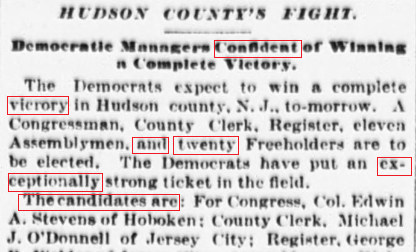
\includegraphics[scale=0.75]{originalimage}
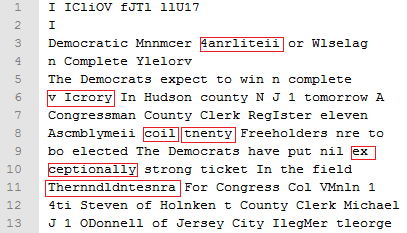
\includegraphics[scale=0.80]{ocr}
\caption{Scanned Image of a Newspaper article (left) and its OCR raw text (right)}
\label{figure:1}
\end{figure}

\begin{description}
 \item[$\bullet$Real word errors] include words that are spelled correctly in the OCR text but still incorrect when compared to the original newspaper article image. For example: In Figure~\ref{figure:1}, the word ``coil"  has been correctly spelled in the OCR text  but should have been ``and" according to the original newspaper article. 
 \item[$\bullet$Non-real word errors] include words that have been misspelled due to some insertion, deletion, substitution or transposition of characters from a word. For eg. In Figure~\ref{figure:1}, the word ``tnenty" in the OCR text has a substitution error (`n' should have been `w') which is actually ``twenty" according to the original newspaper article.
 \item[$\bullet$Non-word errors] include words that have been spelled incorrectly and are a combination of alphabets and numerical characters. For example: In Figure~\ref{figure:1}, the word ``4anrliteii" which is a combination of alphabets and number and should have been ``confident" as per the original newspaper article.
\item[$\bullet$New Line errors] include words that are separated by hyphens where part of a word is written on one text line and remaining part in the next line. For example: In Figure~\ref{figure:1}, the word ``ex-ceptionally" where ``ex" occurs on one line while ``ceptionally" in the next and due to no punctuation in the text, they are treated as separate words in OCR text.
\item[$\bullet$Word Split and Join errors] include words that either get split into one of more parts or some words in a sentence get joined to a make a single word. For example: In Figure~\ref{figure:1}, the word ``Thernndldntesnra" in the OCR text is actually a combination of three words ``The candidates are" while the words ``v Icrory" are actually equivalent to a single word ``victory" when compared with the original news article.
\end{description} 





%\section{Data Preprocessing}
%\label{chapter:data preprocessing} 

 
%This section describes the preprocessing steps applied on the historical news articles.
%The garbled OCR text makes data preprocessing mandatory before application of any text mining algorithms. 

\section{Spelling Correction}

Several kinds of spelling errors exist in the data as described in the previous section. 
%This section first provides a brief review of spelling correction algorithms that exist in literature (Section~\ref{spell:rw});
 This section describes the spelling correction algorithm used in this research  in Section~\ref{spell:algo} and the evaluation algorithm is presented in Section~\ref{spell:sce}.


% DOUBT: Do the following lines need to be removed?
%The garbled OCR dataset  needs to be refined by correcting the text with the help of a human editor manually or automatic spelling corrector. Due to the huge size of dataset, human editing would be extremely time consuming and expensive making it impossible and indicating requirement of a spelling correction technique. 
%The spelling correction of person named entities in the dataset also requires special consideration so that the person named entities with correct spellings get detected as a result which is the main aim of this research.



  
%CHANGES MADE HERE. ADDED A LINE REGARDING PERSONAL NAMES CORRECTION AND MOVED RELATED WORK REGARDING EVALUATION ALGORITHM TO SECTION 4.1.3.
 We use edit distance algorithm for spelling correction because of its speed and ability to correct OCR errors compared to the n-gram approach \cite{chattopadhyaya2013fast}. Context-dependent spelling correction is not used because of unavailability of n-gram words corpus or ground truth dataset containing OCR and true word pairs.
% Our edit distance algorithm also uses an enhanced dictionary for look up to give significance to personal names spelling correction in the dataset. 


\subsection{Spelling Correction Algorithm}
\label{spell:algo}

The Edit Distance algorithm based on Levenshtein distance\cite{levenshtein1966binary} has been used for spelling correction. It is an isolated word correction technique that uses dictionary based-look up method and distance between strings for matching the text and correcting it. An ``edit distance" corresponds to the minimum number of insertions, deletions, and substitutions required to transform one string into another. The algorithm corrects Non-Real Word spelling errors up to an edit distance of 2 , i.e. , it corrects words which have spelling errors that can be corrected by making at most 2 operations of insertion, deletion and substitution of letters in the word. The choice of 2 is governed by the trade off between algorithm runtime and quality of spelling correction. A bigger value improves the spelling correction accuracy but increases the runtime also while a smaller value decreases accuracy and the algorithm runtime.
The spelling corrector has been designed as suggested by Peter Norvig\footnote{ http://norvig.com/spell-correct.html}. The algorithm requires a dictionary which is used to check if each word of the text exists in it or not. If the word already exists in the dictionary then no change is made to the word and if not, then a candidate list of words is created from the word to be corrected by inserting, substituting or deleting up to 2 letters from it.  This list of words is again checked for in the dictionary and returned as suggestions for the word to be corrected. The correction is made with the word formed from lowest edit distance and occurring with more frequency in the dictionary. This makes the edit distance algorithm dependent on the type of dictionary chosen for correction which means the dictionary must be well chosen for spelling correction of a specific document collection. The algorithm runs faster by reading the dictionary only once and keeping a data structure in memory for its word counts which can be referred to whenever a word comes up for correction.

\subsection{Spelling Correction Algorithm Evaluation}
\label{spell:sce}

For evaluation on our dataset, the raw OCR text and OCR text after application of spelling correction algorithm needs to be compared with the original newspaper text. The OCR text is extremely garbled with Word Split and Join errors due to which word-to-word alignment with the original newspaper text is impossible. For this purpose, a novel algorithm called SCE (Spelling Correction Evaluation) based on N-gram approach is proposed for automatic evaluation of the corrected text word-by-word against the manually corrected subset of the news articles dataset. The SCE algorithm can be used for evaluation of spelling correction which is performed using any type of spell correction algorithm.

Following sections describe the evaluation parameters for estimating the performance of Spelling Corrector on the OCR dataset used along with the SCE algorithm:

\subsubsection{Evaluation Parameters}

\begin{description}

 \item[$\bullet$Accuracy]
 The evaluation metric used for measuring the performance of Spelling correction algorithm is Accuracy which requires calculation of number of OCR errors that got corrected when compared to the original scanned newspaper text. The measure has been chosen so as to include the complete text coverage and not just check for words that got corrected after spell correction as in the latter case, the  number of FP and TN get missed which won't give the correct measure of how well the spell corrector works. The formula used for calculating Accuracy is defined by Manning and Schutze,1999 (p.268-269) as follows:

$$Accuracy=  \dfrac{TP+TN} {TP+ FP + TN + FN}$$


where, 

$TP$=Number of True Positives,

$TN$=Number of True Negatives,

 $FP$=Number of False Positives,

 $FN$=Number of False Negatives. 

The aim of the SCE algorithm is to make a word-to-word correspondence between the OCR corrected text and the original OCR text and to mark each token in the OCR text as a $TP$, $FP$, $TN$ or $FN$. Reynaert and Martin\cite{reynaert2008all} suggest a way to define these terms by distinguishing between correct words and incorrect words in the text through the set of non-target, target and selected words and use Precision and Recall evaluation measures for measuring performance of spelling correction. 

According to our spelling corrector, a ``true positive" is said to occur when a word from the OCR text gets corrected and the corrected spelling matches the one in original article text while a ``false positive" occurs if the corrected spelling does not match the corresponding word in the original article text. A ``true negative" occurs when a word does not get corrected by the algorithm as it is already correct and matches the correct word in the original text also. On the other hand, a ``false negative" occurs when the algorithm is unable to correct the word (there is no change in spelling of the word) and it does not match the corresponding word in the original text but should have been corrected.



\item[$\bullet$Time taken for Spelling Correction]
Time is also an essential parameter while measuring the performance of spelling correction. Since the dataset is quite large, it is important that the algorithm does not take too long to correct an article and needs to be parallelized in case it takes more time for correction.


%\item[$\bullet$Person Names Detection Rate(PNDR)]

%The spelling correction algorithm is evaluated on the basis of another parameter which is used to consider the special case of person entity names spelling correction, as the main goal of research is to detect these names with correct spellings.
%Person Names Detection Rate can be defined as the ratio of person names recognized through Named Entity Recognition (NER) before spelling correction process and the total number of person names recognized in the original newspaper articles.

%$$Person Names Detection Rate=\dfrac{ \text{Person Names recognized before/after spelling correction}} {\text{ Person Names recognized in original newspaper articles}} $$

\end{description}

\subsubsection{SCE (Spelling Correction Evaluation) Algorithm}

The SCE algorithm is based on an N-word grams approach. To make the correspondence between corrected and original OCR text, a window of n-word grams in the scanned image text article is considered (Original.txt) which can be seen in a diagrammatic representation in Figure~\ref{figure:2}.

\begin{figure} [!htb]
\centering
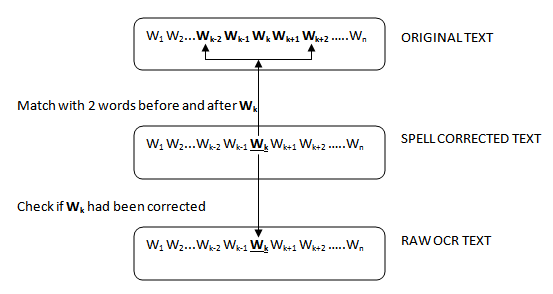
\includegraphics[scale=0.8]{ngram}
\caption{Schematic diagram for alignment of spell corrected article text with original article text for a word $W_{k}$}
\label{figure:2}
\end{figure}
For each token in the spell corrected text (Corrected.txt), the corresponding token  in the scanned text article along with 2 tokens before and 2 tokens after it are considered for alignment\footnote{ The choice of 2 is based on the Word Split and Join errors in the dataset. Choosing n=2 allows a window of words to be considered to make up for the alignment lost because of Word Split and Join errors.}.
If the token being considered matches with any of these words in the scanned text article words window and its spelling has been corrected when compared to the corresponding token in raw OCR text (OCR.txt), then it is marked as a ``True Positive" which is actually rewarding the Spell corrector for making the correct spelling change. A ``False Positive" is marked if it does not match any of the words despite its spelling being corrected. If the token being considered matches any of the words in the words window but no spelling correction has been made for it, then it is marked as a ``True Negative" and if it does not match any word in the window and the spelling corrector also did not correct it, then it is marked as a ``False Negative" as the word got missed by the corrector. 

Several cases could occur like difference in the lengths of linetext between OCR and Original text or while considering the first, second or the last tokens from the Corrected text for which the corresponding word window in Original text needs to be smaller. All such cases have been covered in SCE Algorithm 1 which calls function `MatchWordGrams' (Algorithm2) for these different cases. 

A limitation of the SCE algorithm is that it requires all 3 versions of a newspaper article (Original, Corrected and OCR) to have the same number of lines. In case of difference in the number of lines of text due to some Word Split and Join errors, the words window needs to be extended so as to cover previous and next line texts also for alignment.


\begin{algorithm}[!h]
\caption{SCE Algorithm for Spell Correction}
  \KwIn{Ocr.txt,Corrected.txt,Original.txt}
  \KwOut{Spell Corrector Accuracy }
\SetKwFunction{MatchWordGrams}{MatchWordGrams}%
 $OcrLine$:=a line of text from Ocr.txt\;
 $CorrectedLine$:=a line of text from Corrected.txt\;
 $OriginalLine$:=a line of text from Original.txt\;
 $tp \leftarrow $0  $fp \leftarrow $0 $tn \leftarrow $0 $fn\leftarrow $0\;  
	\For{(int i=0; i $<$ CorrectedLine.length ; i++) }
	{

    \If{(CorrectedLine.length$<$4 $||$ OriginalLine.length$<$4)}
	{		
    	\MatchWordGrams{(OcrLine,CorrectedLine,OriginalLine,0,OriginalLine.length,i)}\; 
	}
    \Else{
   \If {(i==0)}
   {
\MatchWordGrams{(OcrLine,CorrectedLine,OriginalLine,0,3,0)}\;
   }
   \ElseIf{ (i==1)}
   {
\MatchWordGrams{(OcrLine,CorrectedLine,OriginalLine,0,4,1)}\;
   }
	\ElseIf{(i==(CorrectedLine.length-2) $||$ (CorrectedLine.length-1) $||$ (CorrectedLine.length) $||$ (CorrectedLine.length+1))}
	{
\MatchWordGrams{(OcrLine,CorrectedLine,OriginalLine,i-2,OriginalLine.length,i)}\;
	}  
	\ElseIf{(i $>$= CorrectedLine.length+2)}
	{	
\MatchWordGrams{(OcrLine,CorrectedLine,OriginalLine,OriginalLine.length-3,OriginalLine.length,i)}\;	
	}
	\Else
	 {
\MatchWordGrams{(OcrLine,CorrectedLine,OriginalLine,i-2,i+2,i)}\;	
	}	
   }
 }
 	 $Accuracy=(tp+tn)/(tp+tn+fp+fn);$\
\end{algorithm}


\begin{algorithm}[!htb]
\caption{MatchWordGrams Function called by Algorithm 1}
\begin{algorithmic}
\Function {MatchWordGrams}{OcrLine, CorrectedLine, OriginalLine, jstart, jend, i}
  
 \For{(int j=jstart; j$<$jend; j++)}
  {
    \If{ ((CorrectedLine[i].equals(OriginalLine[j]))\&\&(!(OcrLine[i].equals(CorrectedLine[i]))))}
     {
	  $tp=tp+1$\;
	  flag0=false\;
	 \Return $tp$\;
	  }
	\ElseIf{((CorrectedLine[i].equals(OriginalLine[j]))\&\&(OcrLine[i].equals(CorrectedLine[i])))}
	      {
		 $tn=tn+1$\;
		  flag1=false\;
		\Return $tn$\;
	      }
}

	 \If{(!(OcrLine[i].equals(CorrectedLine[i]))\&\&flag0==true)}
	 {
		    $fp=fp+1$\;
		   \Return $fp$\;
            }
	 
	 \ElseIf{((OcrLine[i].equals(CorrectedLine[i])) \&\& flag1==true)}
	 {
		    $fn=fn+1$\;
		   \Return $fn$\;
	 }
\EndFunction
\end{algorithmic}
\end{algorithm}


\clearpage


\begin{figure} [!htb]
\begin{center}
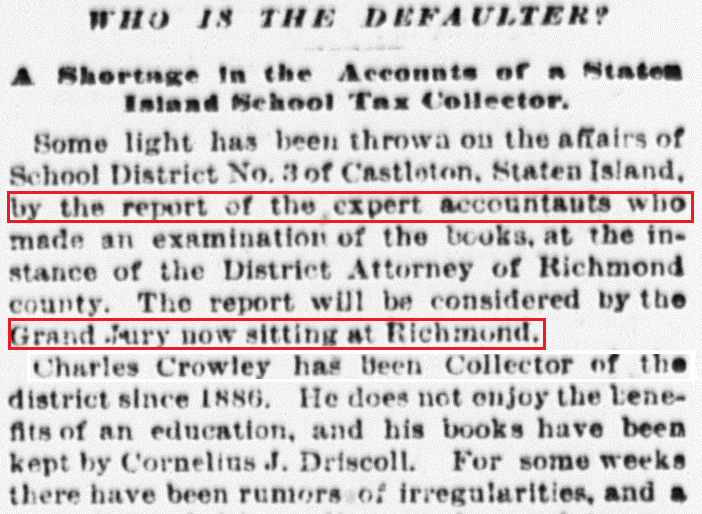
\includegraphics[scale=0.4]{img3}
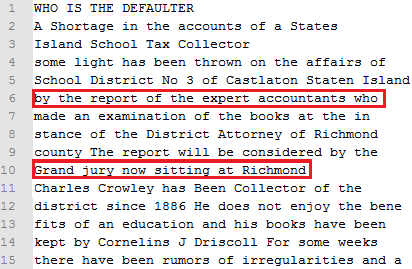
\includegraphics[scale=0.75]{originalimg3}
\caption{Scanned image of a newspaper article (left) along with its original text (right)}
\label{figure:3}
\end{center}
\end{figure}


\begin{figure} [!htb]
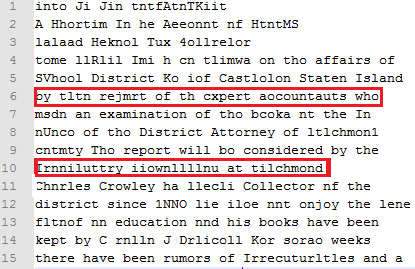
\includegraphics[scale=0.75]{ocr3}
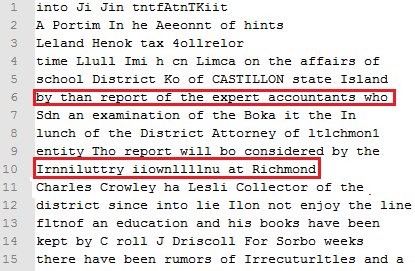
\includegraphics[scale=0.75]{corrected3}
\caption{OCR raw text (left) and Spell corrected text (right) of the article}
\label{figure:4}
\end{figure} 


\textbf{An Example}


Working of the SCE algorithm can be demonstrated with the help of the following example:
Consider 3 versions of a scanned image of a newspaper article,  the original text of the scanned image in Figure~\ref{figure:3} and the raw OCR text and the corrected text (after spell correction) in Figure~\ref{figure:4}. As highlighted in the figures, for line 6 the line texts are:

 OcrLine= \textit{by tltn rejmrt of th cepert aocountauts who}

CorrectedLine= \textit{by than report of the expert accountants who}

OriginalLine= \textit{by the report of the expert accountants who} 

Here, for each token of CorrectedLine, we find its index and call the MatchWordGrams function accordingly. For the first token `by' at index i=0 in CorrectedLine, we consider the word window to be ``by the report" (index j=0 to 2) in OriginalLine by matching iteratively with each token to see if there is a match and also if there has been a spelling correction by comparing with the corresponding token in OcrLine. Here, no change was made to the spelling of `by' and it matches with a word in words window, so it is marked as a FN. For the second token `than' at index i=1, we consider the word window to be ``by the report of" (index j=0 to 3) for which there is no match in the window but there has been a spelling correction from `tltn' to `than', which implies the correction was wrong and the token is marked as a $FP$. For the third token `report' at index i=2, we consider the window as ``by the report of the" (index j=0 to 4) in Original Line and find that there is a match in the word window and there has been a spelling correction too from `rejmrt' to `report' which makes this token a $TP$. Similarly, rest of the tokens get marked for each line in the Corrected.txt. 

Another example can be considered from Line 10 in Figure~\ref{figure:3} and Figure~\ref{figure:4} where the number of tokens is different in CorrectedLine and OriginalLine. In such a case, direct alignment between tokens is not possible because of which the words window becomes useful. Here, when the last token `Richmond' of CorrectedLine is considered at index i=3, the corresponding words window becomes ``Jury now sitting at Richmond" (index j=1 to 5) for which there is a match in the words windows and corresponding spelling has also been changed from `tilchmond' to `Richmond' which makes it a $TP$. Had the word window not been considered, the corresponding token at index j=3 in OriginalLine would have been chosen as `sitting' which would have resulted in a $FP$. 
   

\section{Empirical Evaluation and Results}
%\subsection{Spelling Correction Algorithm Evaluation Results}
%\label{spell:eval}



\subsection{Data Source} 

The dataset has been taken from Chronicling America.
\noindent \emph{Chronicling
America}\footnote{\texttt{http://chroniclingamerica.loc.gov/}} is an
initiative of the National Endowment for Humanities (NEH) and the
Library of Congress (LC) whose goal is to develop an online,
searchable database of historically significant newspapers between
1836 and 1922. The New York Public Library (NYPL) is part of this
initiative and has scanned 200,000 newspaper pages published between
1890 and 1920 from microfilm.

In order to make a newspaper available for searching on the Internet,
the following processes used in \cite{dutta2011learning} must take place: (1) the microfilm copy or
paper original is scanned; (2) master and Web image files are
generated; (3) metadata is assigned for each page to improve the
search capability of the newspaper; (4) OCR software is run over high
resolution images to create searchable full text and (5) OCR text,
images, and metadata are imported into a digital library software
program. The scanned newspaper holdings of the NYPL offers a wealth of
data and opinion for researchers and historians.

The newspaper titles and digitized pages available through the
Chronicling America website can be searched using the OpenSearch
protocol\footnote{\texttt{http://www.opensearch.org/Home}}.
Unfortunately, the current search facilities are rudimentary and
irrelevant documents are often more highly ranked than relevant ones.
The newspapers are scanned on a page-by-page basis and article level
segmentation is poor or non-existent; the OCR scanning process is far
from perfect and the documents generated from it contains a large
amount of garbled text. In a bid to serve its patrons better, the New
York Public Library employed human annotators to clean headlines of
articles and text, but the process of manually reading all the old
newspapers article-by-article and cleaning them soon became very
expensive. 
\subsection{Data Statistics}
The OCR text available from Chronicling America website is on a page by page level and no article level segmentation is provided. OCR text dataset is therefore, taken from a PostgreSQL database where article level segmentation of page-level OCR text from Chronicling America is available for two months of articles of ``The Sun" newspaper from November-December 1894 consisting of 14020 news articles with a total of 8,403,844 tokens. The newspaper database ER diagram \footnote{https://power.ldeo.columbia.edu/twiki/pub/Incubator/BodhiDBDesign/Final ERD.pdf }
is used to extract the required articles text from the database by dumping complete dataset and extracting individual articles linetext based on their unique ID. The individual text articles generated from the database do not have any punctuation and contain a large amount of garbled text containing above mentioned OCR errors.


\noindent \textbf{Aims: }The aim of our experiments is to answer the following question:
How good is the spell corrector? The metrics for evaluation are accuracy and time to correct the text.
 
%\item \textbf{Question 2: }How good is the Person Names Detection Rate? The metric for evaluation is PNDR. 


\subsection{Experimental Procedure and Results}
\noindent \textbf{Materials: }
The spelling correction algorithm is used to correct all the 14020 OCR raw text articles in the dataset. The dictionary used for look-up is a concatenation of several public domain books from Project Gutenberg and lists of most frequent words from Wiktionary and the British National Corpus\footnote{http://norvig.com/big.txt}. This is augmented with a large people names list which is obtained  by running Stanford NER-CRF parser on subsets of the ClueWeb12 dataset made available in the TREC 2013 Crowdsourcing Track\footnote{http://boston.lti.cs.cmu.edu/clueweb12/TRECcrowdsourcing2013/}. This enhanced dictionary has been used to give special consideration to correction of person names in the dataset.

\noindent \textbf{Methods: }
In order to answer our research question fo checking the performance of spell corrector, we do the following: 

3 versions of each newspaper article are required: OCR raw text, spelling corrector corrected text and the original scanned newspaper article text. Since the dataset is quite large (14020) and it is not possible to get original text of each of these newspaper images, a smaller number of articles are chosen to study the results of spelling correction. 50 scanned newspaper images are taken and an online OCR \footnote{www.onlineocr.net} is run on them followed by some manual correction to get the original articles text. Accuracy can then be calculated for all 3 versions of 50 newspaper articles using the SCE algorithm by marking each word in the OCR text article as a $TP$, $FP$, $TN$ or $FN$. 

%In order to answer \textbf{Question 2} we do the following: 
%% AAYUSHEE CHECK--DONE
%\begin{enumerate}
%\item Person Name Detection from raw OCR (\textbf{Baseline: }) The NER is run on the raw garbled OCR text.
%\item Person Name Detection from spell corrected text (\textbf{PND+Spell Correction+Simple Dictionary: })The NER is run on the spell corrected (using the edit distance algorithm) OCR text without the people names list in the dictionary.
%\item Person Name Detection from spell corrected text with enhanced dictionary (\textbf{PND+Spell Correction+Enhanced Dictionary: }) The NER is run on the spell corrected (using the edit distance algorithm) OCR text with the enhanced people names list in the dictionary.

%\end{enumerate}

\noindent \textbf{Results: }
The spelling corrector takes 9 seconds on an average to correct the newspaper OCR articles. It takes a total of 36 hours to run on 14020 articles.
The spelling corrector shows an Accuracy of $72.7 \%$  when corrected text is compared to OCR text and original article text using our SCE algorithm. We believe that the results are less accurate due to the presence of a large number of Non-word, New Line, Word Split and Join errors in the OCR data which can not be corrected by the spelling correction algorithm used for this research.




%But the spelling correction is useful in terms of Person Names Detection Rate \textit{(PNDR)}. Following are the statistics obtained for \textit{PNDR}:

%\textit{PNDR} for \textbf{Baseline: }: 71.5\% 

%\textit{PNDR} for \textbf{PND+Spell Correction+Simple Dictionary: }: 63.3\% 

%\textit{PNDR} for \textbf{PND+Spell Correction+Enhanced Dictionary: }: 85.5\% 

%These statistics indicate that spelling correction using an extended dictionary for personal names is useful for detecting person names from the garbled newspaper articles and the results are dependent on the type of dictionary being used for spell correction.
 %Table~\ref{table:pndr} shows some of the person names recognized while calculation of PNDR for each case. The reason for PNDR going down after spell correction with simple dictionary is demonstrated from the table as unnecessary spelling corrections are made while using this dictionary. On the other hand, since the enhanced dictionary contains several person names and no unnecessary spelling corrections are made, more persons name are recognized in this case when compared to the original text leading to a much higher PNDR. 

\section{Discussion and Future Work}
\label{spell:discussion}

\begin{description}
\item[$\bullet$]\noindent
We believe a better accuracy of spell correction can be obtained by correcting the New Line errors in the articles. This can be done by checking for if the word at last index of a text line or the word at first index of the next text line is a word not present in the dictionary and combining the two and checking again in the dictionary for a valid word. The new word, if present in the dictionary can be replaced by the two words from which it is formed thereby removing the New Line error. 
\item[$\bullet$]\noindent Similar approach can be applied for Word Split and Join errors but would require each word of an article not present in the dictionary to be analyzed along with some window of words before and after it to make a correction. 
\item[$\bullet$]\noindent Choice of a dictionary for the edit distance algorithm affects the results as indicated by improvement in PNDR while using an enhanced person names dictionary. We believe using a dictionary with historical terms, places and people names can certainly perform spelling correction better and improve the accuracy also.
\item[$\bullet$] \noindent 
Our spell corrector corrects Non-Real Word errors by focusing on isolated words in the dataset. Other spelling correction algorithms like context dependent spelling correction can also used to correct the dataset and measure accuracy using our SCE algorithm along with other evaluation parameters to compare among multiple algorithms and decide which one suits the dataset better and gives best accuracy. 
\end{description}



\section{Acknowledgement}


%The body of the paper should be divided into sections. Use 12-point Time New Roman font for the text of each section.
%The body of the paper should be single-spaced, justified, and in one-column format. Leave one-line spacing between paragraphs.
%The completed paper, including graphics and references, cannot exceed six (6) pages.
%Tables, figures, and equations should be included in the main text. Tables and figures must be centered. Equation numbers must be f%lush right.

%\begin{equation}
 %y = x^2 + z^2
%\end{equation}

%References should be numbered and listed at the end of the paper in the section References.
%Within the text, they should be cited by the corresponding numbers, enclosed in brackets,
%e.g., \cite{ Baydogan13bof}, or \cite{ Baydogan13bof,cortina1993interaction,jebara04ppk}  for multiple references.
%Examples of reference formats are shown below.
%\begin{table}[!h]
%\centering
%\begin{tabular}{|r|r|r|r|}
 % \hline
  %1 & 0.8151 & 0.9401 & 0.4640 \\   \hline
  %2 & 0.5028 & 0.6623 & 0.5464 \\   \hline
  %3 & 0.1423 & 0.0884 & 0.0465 \\   \hline
  %4 & 0.3435 & 0.2900 & 0.7783 \\   \hline
%\end{tabular}
%\caption{Caption}
%\end{table}

\bibliography{aayushee}


\end{document} 